%% neuro_concepts.tex
A large part of the contribution of this thesis consists of identifying relevant findings from neuroscience and adapting them to a deep learning setting.
The identified concepts and the link between the two disciplines are described in this chapter.
This chapter presents only one possible interpretation for implementing neuroscientific concepts in the context of deep learning; alternative interpretations might also be promising.
Concrete implementations of the concepts presented in this chapter can be found in \chref{vertical_self_org} and \chref{horizontal_self_org}.

The following is discussed in this chapter:
\secref{neuro_concepts_discrepancy} describes the discrepancy between biological learning and deep learning and points out why it is hard to adapt the biological concept to algorithms. Next, \secref{neuro_concepts_self_org} self-organisation is presented as one of the fundamental concepts for natural intelligence and a possible implementation is proposed. Afterwards, net fragments are discussed in \secref{neuro_concepts_net_fragments}. Next, \secref{neuro_concepts_lateral_connections} proposes a method of how lateral connections can be interpreted in a deep learning setting. Finally, \secref{neuro_concepts_others} points out other promising principles that are not implemented in the course of this thesis but might be helpful in future work.


\section{The Discrepancy}\seclbl{neuro_concepts_discrepancy}
The human brain inspired deep learning, and consequently, many essential components of a deep learning model are named after their biological counterparts. Nevertheless, this linkage is misleading: both systems work fundamentally differently, and many concepts cannot be transferred directly.
This experience is one of the author's most important but unfortunate findings, especially as it was only made towards the end of the thesis (and after multiple failed attempts that are not written down in this document). This confusion of terminology between deep learning concepts and insights from neuroscience hinders and, in some cases, prevents the development and implementation of novel concepts\sidenote{a lesson that probably has to be learnt by anyone researching along the ridge of these two fields}. 

In the biological context, neurons are often discussed as the main component of the nervous tissue and, thus, the nervous system.
A neuron is a well-defined cell consisting of components such as the cell body, dendrites, and an axon communicating with other neurons via synapses (c.f. \secref{neurons}).
Consequently, in the neuroscience context, it is clearly defined what a neuron is. In fact, many of the theories in neuroscience are based on how neurons behave in various circumstances (see the following chapters). 

In the field of deep learning, this definition is much vaguer. It could even be argued that neural networks do not contain neurons: Deep learning systems model and optimise weight parameters. Admittedly, multiplying a weight matrix $\boldsymbol{w}$ with input data $\boldsymbol{x}$ and adding a bias $\boldsymbol{b}$, i.e. $\boldsymbol{w} \cdot \boldsymbol{x} + \boldsymbol{b}$, can be interpreted as a kind of modelling of a neuron\sidenote{however, also in this case, weights and not neurons are modelled explicitly} (c.f. Section \secref{ann}). 
However, modern network architectures are typically not solely based on this fully-connected modelling pattern.
Modern deep learning architectures for computer vision are usually based on either convolutional operations (c.f. \secref{cnns}) or attention mechanisms \sidecite{Dosovitskiy_Beyer_Kolesnikov_Weissenborn_Zhai_Unterthiner_Dehghani_Minderer_Heigold_Gelly_2021}. The convolutional and pooling operations of CNNs cannot properly be modelled with neurons. The same applies to the attention mechanism of vision transformers. Furthermore, both architectures use various other concepts that have been shown to improve results and computation efficiency, such as normalisation layers, etc.
As a result, findings from neuroscience are often based on the investigation of neurons or neuron structures, and consequently, the theories and findings derived from them cannot be transferred to deep learning settings in a simple way, as neural network model weights, which are processed by various mathematical functions.

Another fundamental difference is the interaction between the neurons. Biological neurons fire electrical impulses when they are sufficiently excited. The synaptic signals generated can be either excitatory or inhibitory. If the biological network is frozen in a certain state, it could be argued that the neurons are binary (excited or not excited). In reality, however, this process is much more complex: neurons communicate in temporal patterns of spikes.
Artificial neurons, on the other hand (or, more precisely, the result of the matrix operation, often referred to as a neuron), can take on any floating point number as a ``state'' and thus represent an infinite number of states in a frozen state. On the other hand, artificial neurons have no temporal dynamics. Thus, a large part of the intelligence of biological networks lies in the temporal pattern of the spikes, which are not taken into account by artificial neural networks (and cannot be modelled efficiently due to the clock-gated processing of modern computing infrastructure). These facts make it extremely difficult to link biological and artificial networks: If a frozen state of both networks is discussed, then a fundamental building block of biological neurons is missing, i.e. the temporal aspect. If, on the other hand, time dynamics are taken into account, then deep learning networks are not suitable, and spiking networks have to be used.

Although biological and artificial neuronal networks are fundamentally different in many aspects, there are also many similarities, and biological findings can serve as a source of inspiration. However, this section should make clear that these sources of inspiration are to be interpreted somewhat abstractly and cannot be implemented in the same form as in the human brain. Many failed experiments that are not documented in this thesis have failed because their implementation was too strongly oriented towards the biological concept. Therefore, in the following sections, various concepts are discussed, and intuitions are given on how these concepts can be interpreted in a deep learning setting without time dynamics but with complex neuron states.

\section{Self-Organisation}\seclbl{neuro_concepts_self_org}
It is known that large parts of the human brain are self-organising \sidecite{kelso1995dynamic}.
Self-organisation is the process by which systems consisting of many units acquire their function through local interaction and without interference from an external supervisory system.
Recently, renowned scientists \sidecite{von_der_Malsburg_Stadelmann_Grewe_2022} put forward the hypothesis that this process of self-organisation is \emph{the} key mechanism of natural intelligence.
Dresp \sidecite{Dresp2020SevenPO} describes seven clearly identified properties of self-organisation in the human brain: (i) modular connectivity, (ii) unsupervised learning, (iii) adaptive ability, (iv) functional resiliency, (v) functional plasticity, (vi) from-local-to-global functional organisation, and (vii) dynamic system growth.
However, it is not obvious how these insights from neuroscience can be integrated into a deep learning framework.

Deep learning networks are usually optimised with end-to-end backpropagation of error.
Thus, the entire network is optimised for a specific target.
This is a violation of the self-organisation principle as a global update algorithm (i.e. the optimiser) adjusts all network weights to minimise a global target function.


\begin{claim}
	End-to-end backpropagation of error violates the principle of self-organisation. Self-organisation in neural networks requires dividing the network into smaller units that are optimised independently of each other.
\end{claim}

In fact, the plausibility of backpropagation of error for explaining how the brain works was questioned soon after it was published \sidecite{Crick_1989, Grossberg_1987}.
The biologically most plausible learning algorithm is Hebbian learning (c.f. Section \secref{hebbian}) and its variants, such as contrastive Hebbian learning \sidecite{Movellan_1991}.
However, Hebbian learning is not well suited for learning good image representation if a network is trained from scratch. However, it might be more promising for processing already retrieved representations (c.f. Appendix \chref{exp_hebb_learning}).

Besides Hebbian learning, many alternative and biologically more plausible algorithms have been proposed, such as the feedback alignment (FA) algorithm \sidecite{Lillicrap_Cownden_Tweed_Akerman_2016}, generalised recirculation \sidecite{O_Reilly_1996}, as well as target propagation (TP) \sidecite{Le__Cun_1986} (c.f. \secref{alt_train_algo}).
However, Bartunov et al. \sidecite{Bartunov_Santoro_Richards_Marris_Hinton_Lillicrap_2018} have demonstrated that these algorithms do not scale to large vision datasets such as ImageNet \cite{deng2009imagenet}, and only work for smaller datasets such as MNIST \cite{MNIST}, and CIFAR-10 \cite{cifar_10}.
The only algorithms that scale well and rely on local updates only use proxy objective functions (c.f. Section \secref*{alt_train_algo}).
Thus, the use of proxy objective functions\sidenote{proxy objective functions are loss functions that are only applied to local units of a system} seems promising; the weight updates are done in separate local units, yet the power of current deep learning training algorithms can be exploited. Thus, it allows to create complex systems that scale to large datasets while being based on local units interacting with each other.

\begin{implementation}
	Instead of using end-to-end backpropagation of error to optimise the whole system according to a single global objective function, proxy objective functions can be applied to local units. Thus, self-organisation takes place through optimising multiple local units instead of optimising a single system.
\end{implementation}

Another ambiguity is the definition of local units in a deep learning setting.
One of the strengths of deep learning systems is that matrix multiplications allow to calculate the layer's outputs in one step.
Calculating each neuron activity separately, on the other hand, would be very inefficient.
Therefore, the smallest meaningful unit for local updates is a layer and not a single neuron.
In this thesis, the layers of a network are optimised separately with proxy objective functions. Doing so makes the local units small but allows optimising them efficiently.
If a neural network is visualised layer-wise from left to right, the self-organising units (i.e. the layers) line up horizontally. That is why layer-wise self-organisation is referred to as ``horizontal self-organisation'' in this thesis (c.f. \figref{horizontal_vertical_self_org}).

\begin{implementation}
	Self-organisation takes place within local units. A local unit can be a part of a model, such as a layer.
	In this thesis,  optimising layers individually with proxy objective functions is called horizontal self-organisation.
\end{implementation}

\begin{figure}[h]
    \centering
    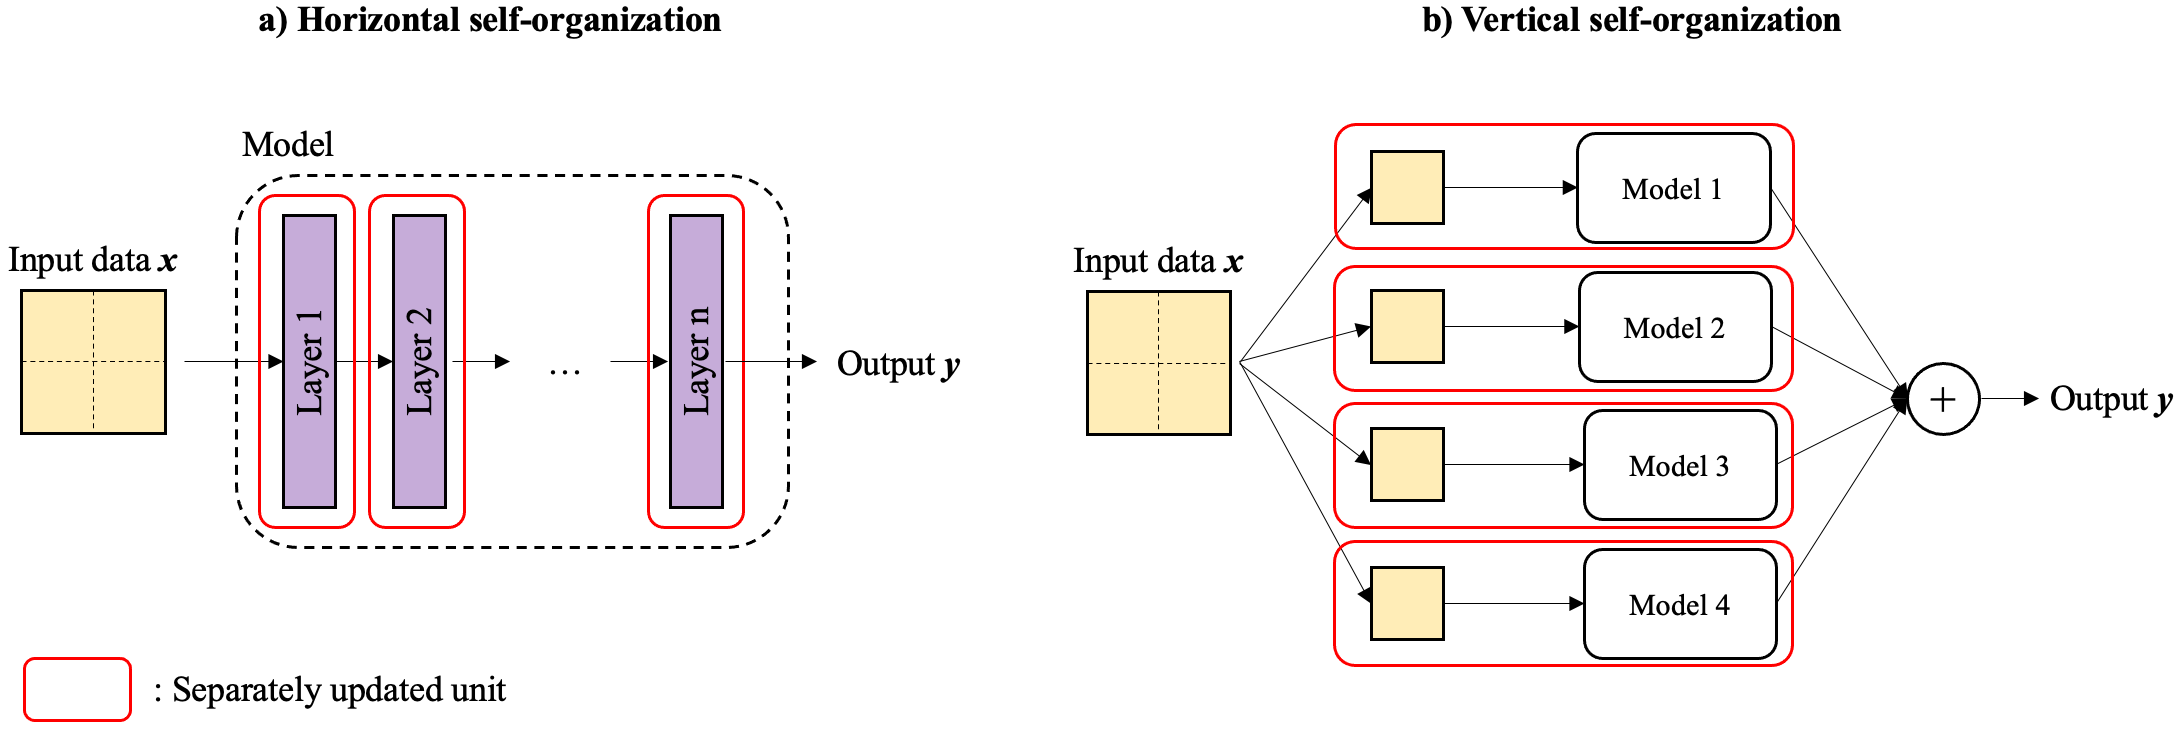
\includegraphics[width=0.99\textwidth]{horizontal_vertical_self_org}
     \caption[Overview of horizontal and vertical self-organisation]{Two ways to build self-organising units: Self-organisation can either take place horizontally (i.e. layer-wise) within a model (a) or vertically by splitting the data into patches and processing them with independent units (b). The self-organising units are marked with a red frame.}
\end{figure}
 
A second type of self-organisation is not to split the model into separate units but to split the data.
The input data can be divided into smaller patches and be processed by independent units (i.e. models).
It is important that one model does not process the entire set of existing patches, as is the case with the vision transformer \sidecite{Dosovitskiy_Beyer_Kolesnikov_Weissenborn_Zhai_Unterthiner_Dehghani_Minderer_Heigold_Gelly_2021}. If only one model is used, there would again be an end-to-end backpropagation of error on a single unit.
However, if a graph of independent models processes the patches, each model can be considered a self-organising unit.
In this thesis, this kind of self-organisation is called  ``vertical self-organisation'' (c.f.  \figref{horizontal_vertical_self_org}).

\begin{implementation}
	A second type of self-organising unit can be a model that processes a subset of input data that is not shared with other models. In this thesis, this type of self-organisation is called vertical self-organisation.
\end{implementation}


\section{Net Fragments}\seclbl{neuro_concepts_net_fragments}
Another fundamental principle for intelligence, according to von der Malsburg et al. \sidecite{von_der_Malsburg_Stadelmann_Grewe_2022}, is that neurons form net fragments (a.k.a. sub-networks) that represent features of objects (c.f. \secref{natural_intelligence}).
For example, some net fragments may represent shapes and structures while a multitude of such net fragments together represents objects such as persons or entire scenes.
Net fragments are a compositional data structure: Some low-level features can be composed into a higher-level feature, and multiple higher-level features represent an entire object.
To some extent, neural networks do this as well; data is fed into the network, the first layer extracts some low-level patterns, and the subsequent layers combine these patterns in higher-level features hierarchically.
However, there is one big difference: The features used to fulfil a specific task, such as classification, are extracted from the latent space of \emph{one} single layer.
On the other hand, net fragments in the human brain are not believed to be present at a specific layer but to be built up over multiple neurons and over a short period of time.

\begin{claim}
	Net fragments are represented by groups of neurons and their activity over several time-dependent spikes. In addition, several net fragments can be combined to form higher-level fragments. Thus, objects are not represented by a single neuron but by all neurons across all layers that were activated due to this object.
\end{claim}

Deep learning models are not based on time-dependent spikes of neurons that compose features to more complex features.
However, a time step could be interpreted as a forward step from one layer to the next within a network of layers.
Thus, net fragments would be the activation of multiple layers.
This interpretation is also in line with the compositional property of net fragments.
Low-level features that are detected within the first layers activate higher-level features in subsequent layers.
An object, however, is not represented in the last layer of a neural network but through all activations within the network.
Thus, representations of objects cannot be extracted from a single but from multiple layers.
Intuitively, this seems promising:
For example, auto-regressive models applied to speech capture different information at different layers of the network \sidecite{chung19_interspeech}.
While the first layers contain more information to distinguish speakers, representations in later layers provide more phonetic content.
Thus, extracting information from several layers could lead to representations containing more relevant information.

\begin{implementation}
	Net fragments cannot be extracted from one single layer. Therefore, the representations of an image are extracted from multiple layers.
\end{implementation}

In the human brain, distinct groups of neurons represent specific net fragments.
This means that neurons are only active when the corresponding feature is present in the input and are inactive otherwise.
Moreover, the features represented by the neurons should be meaningful\sidenote{interpretable in the sense that a neuron is active if a specific feature is present and inactive otherwise} and consequently not active for every existing object.
This inevitably leads to sparse and diverse activations.
The activations are sparse and diverse because the object in the image consists of only a small subset of all learned features. Thus, only a small subset of the neurons should be active for a given object.
When the input changes and a different object is shown to the model, also the set of active neurons should change.

\begin{claim}
	The activation patterns of neurons that represent net fragments must be sparse and diverse to obtain meaningful activation patterns.
\end{claim}

The extent to which neuronal networks contain or can produce net fragments with meaningful activation patterns is investigated in detail in a preliminary study.
The methodology used and an in-depth evaluation is described in the appendix in \chref{net_fragments}.
In summary, it was found that neural networks do not contain net fragments with meaningful activation patterns by default. Typically, some neurons are always active regardless of the input data and encode most of the input information in their activation strength.
Other neurons, however, are never active and are, therefore, not needed by the network.
If, on the other hand, a sparsity and diversity constraint is added, net fragments can be identified in the neuron's activation patterns.

\begin{implementation}
	Sparse and diverse activation patterns can be obtained by imposing sparsity and diversity constraints to the objective function of the model.
\end{implementation}

However, sparsity and diversity constraints are mainly necessary to obtain meaningful and more robust activation patterns.
They are not necessary, for example,  to obtain better classification performance.
An alternative that leads to robust and meaningful activations as well is to model the net fragments as a probability distribution.
For example, variational autoencoders (c.f. \secref{visual_rep_learning}) model their latent space as a multivariate Gaussian distribution.

%Especially for models based on horizontal self-organisation, it seems important to impose these constraints on all layers.
%For models with vertical self-organisation, on the other hand, these constraints do not need to be applied to all layers, as long as there are enough models that can only see very small input patches. In this case, a sub-model can only recognise a very spatially-limited feature, which corresponds to a low-level feature. In order to recognise higher-level features or whole objects, interaction with neighbouring sub-models is necessary.
%Thus, net fragments are composed over several sub-models.
%In this case, it is sufficient to impose the constraints to the function that composes the the representation of the sub-models to higher-level net fragments or to objects.


\subsection{Sparsity}\seclbl{neuro_concepts_sparsity}
Sparistiy is an important principle in biological networks.
Presumably, this is because the neurons in the brain can be inhibitory or excitatory by firing spikes at different time intervals and thus have a binary state (i.e. active or inactive). Artificial neurons, on the other hand, use a floating point number as an internal state and can thus represent an infinite number of different states.
Thus, an artificial neuron can represent many different things, while the biological neuron is responsible for specific features.
Therefore, the activations of biological neurons \emph{must be} sparse, while the activations of artificial neurons \emph{do not have to be} sparse (but being sparse has also advantages for artificial neurons; see below).

Sparsity is deeply embedded in the biological learning process.
For example, in the visual cortex of mice are more than 75\% of the neurons active before the first opening of the eyes, 36\% after the opening of the eyes and only 12\% in adulthood \sidecite{Rochefort_Garaschuk_Milos_Narushima_Marandi_Pichler_Kovalchuk_Konnerth_2009}.
Thus, a sparsification of neuronal activations takes place through visual experience.
In the field of deep learning, sparsity is often interpreted in two different forms; sparse weight matrices and sparse activation matrices.
Sparse weight matrices are often chosen to make models smaller or to increase inference speed \sidecite{Louizos_Welling_Kingma_2018, Hoefler_Alistarh_Ben_Nun_Dryden_Peste_2021}.
From a biological point of view, this process of first creating an extensive network and then shrinking it is not plausible\sidenote{otherwise, we would have a large brain at the beginning, which becomes smaller by factors with time}.
Sparse activations, on the other hand, can increase robustness \cite{Panousis_Chatzis_Theodoridis_2021}.
Intuitively, sparse activations enforce that only the most relevant information is passed to the subsequent layer.
Furthermore, combining sparsity with diversity can help to obtain better interpretable activations (c.f. appendix \chref{net_fragments}).

\section{Lateral Connections}\seclbl{neuro_concepts_lateral_connections}
In addition to forward connections, also lateral connections are located in the visual cortex \sidecite{gilbert1990lateral}.
Thus, the biological neurons are connected to the neurons in the subsequent layer and within the same layer.
Von der Malsburg et al. \cite{von_der_Malsburg_Stadelmann_Grewe_2022} describe that lateral connections help active neurons to support each other in order to remain active:
Initially, many neurons are active, but relatively quickly, a part of the neuron becomes inactive, and only those neurons that support themselves remain active. In this way, lateral connections can lead to the emergence of high-level features from initial activations.

\begin{claim}
	Lateral connections allow active neurons to support each other to remain active.
\end{claim}

Neural networks lack this time dynamic, and neurons do not suddenly become inactive during a forward pass. 
In addition, initial experiments have shown that performance does not improve when the activation maps of neural networks are sparsified over several steps.
One assumption is that all information is already contained in the data at the beginning, and the same sparsified activations can also be generated in one initial step.

However, the lateral support between neurons seems promising if the input changes slightly:
An activation map can be calculated for a given input image. Then, in the next step, the input can be slightly changed through data augmentation to obtain another activation map from the same image. Thus, the network receives different views of the same image and generates different activation maps of the same image. In every step, the model can decide whether the activation map from the previous step was correct or if the activation map should be updated.

\begin{figure}[h]
    \centering
    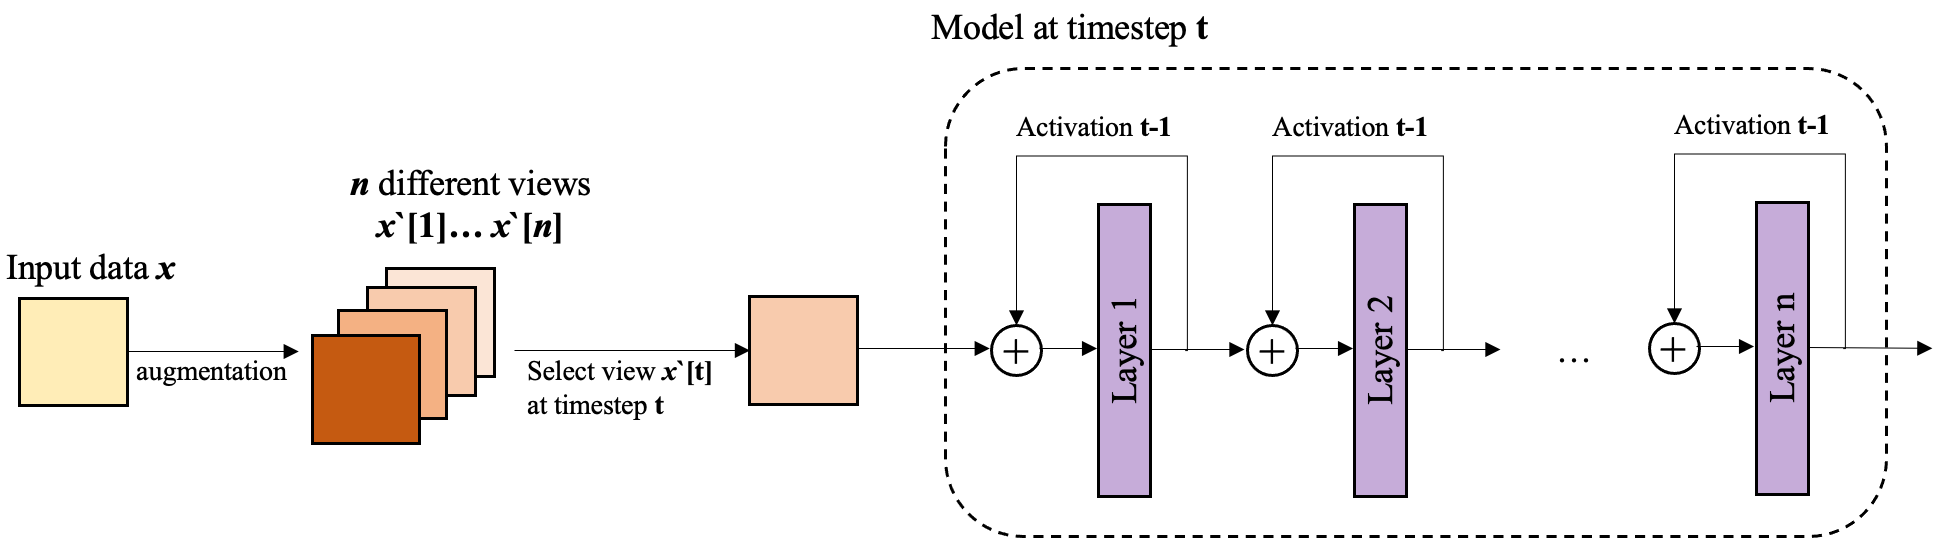
\includegraphics[width=0.99\textwidth]{lateral_connections}
    \caption[Illustrative network architecture of a model with lateral connections]{An illustrative network architecture of a model with lateral connections: An input sample $\boldsymbol{x}$ is augmented $n$ times to obtain $n$ different views $\boldsymbol{x}'[1], ..., \boldsymbol{x}'[n]$ of the same sample. At every time-step $t$, the sample $\boldsymbol{x}'[t]$ is fed through the model. Each layer receives the activation map of the previous layer as input as well as its own activation maps from the previous time-step $t-1$.}
    \figlbl{lateral_connections}
\end{figure}

This can be implemented by interpreting the lateral connection as a recurrent connection.
An illustrative architecture of such a model is shown in \figref{lateral_connections}.
A data sample $\boldsymbol{x}$ can be augmented with data augmentation methods $n$ times to obtain $n$ different views $\boldsymbol{x}'[1], ..., \boldsymbol{x}'[n]$ of the input sample.
Afterwards, the $n$ views are iteratively fed into the model.
At every time-step $t$, the model calculates an activation map $\boldsymbol{a}^{[l]}[t]$ for each layer $l$.
If $t>1$, the input of the layer $l$ is not only the activation map of the layer $l-1$ but also the activation map of the previous time-step $\boldsymbol{a}^{[l]}[t-1]$.
The activation map of the previous time-step is stored $\boldsymbol{a}^{[l]}[t-1]$ by the recurrent (lateral) connection.
Thus, the activation map $\boldsymbol{a}^{[l]}[t]$ is not only calculated based on the activation map of the previous layer $\boldsymbol{a}^{[l-1]}[t-1]$ but also based on the activation map of the previous time-step $\boldsymbol{a}^{[l]}[t-1]$.
Lateral connections allow each layer to preserve the activation map $\boldsymbol{a}^{[l]}[t-1]$ from the previous time-step or to correct it based on a slightly different input $\boldsymbol{a}^{[l-1]}[t]$ from the previous layer. The lateral connections thus support the activations within a layer; a layer can look at several inputs and decide which features are present over several time-steps, thus supporting activated features.

\begin{implementation}
	A lateral connection can be implemented as a recurrent connection that ``stores'' the layer's activation of a previous time-step.
	If the same input is present for several time steps in a slightly augmented version, the layers can keep or correct their previous activation maps (lateral support).
\end{implementation}

With vertical self-organisation, the lateral connections can be implemented as recurrent connections within layers and as connections between the sub-models.
In this case, each sub-model extracts a distinct low-level feature.
Based on this feature, a guess can be made as to which higher-level feature or object the extracted feature belongs to.
This guess can be supported or rejected through communication with neighbouring sub-models.
Thus, the lateral connections can be used as a ``support channel'' or ``communication channel'' between sub-models. 

\begin{implementation}
	In the case of vertical self-organisation, a lateral connection can be implemented as a connection between sub-models to vote for which high-level feature or object is represented in the image. Either the prediction of a model can be supported by neighbouring models or rejected.
\end{implementation}


\section{Other Principles}\seclbl{neuro_concepts_others}
Other important principles that are considered promising are a \emph{continuous input} signal and an \emph{embodiment} of the agent.
However, implementing such an interaction between an agent and an outside world is out of scope for this thesis but might be interesting for future work.

The visual cortex receives a continuous input signal.
This allows the tracking of moving objects and enables an object to be perceived from different angles. Since the object change between the captured frames is small, it can be determined that it is always the same object instance and consequently mapped to the same mental object prototype of a world model.

An ANN, on the other hand, is typically trained on samples that have little relation to each other.
When the system is trained on images, each frame is different; with videos, each sequence of frames is different.
Continuous input might help to get a better representation of objects through self-supervised learning.
Suppose an input is continuous and shows the same object from different angles or in different transformations (e.g. stretching), and it can be inferred that it is the same object. In that case, the object representations derived from this continuous stream can be homogenised.
These principles are already applied to some extent by self-supervised learning systems for computer vision.
In contrastive learning, a popular form of self-supervised learning, two different views are derived from one image by data augmentation, and their representations are then pushed closed together in the feature space \sidecite{chen2020simple, chen2020big, caron2020unsupervised}.
However, this paradigm is still quite limited since only two views of the same scene and not the continuous transformation of an object are presented to the learning system.

\begin{claim}
	A continuous input stream can help to build a better representation of objects, especially if the objects are slightly transformed between captured frames or if the point of view changes continuously and smoothly.
\end{claim}


In the nervous system, efference copies of motor signals in the form of neuronal activities are directly sent to the brain’s sensory system \sidecite{Keller_Bonhoeffer_Hübener_2012}.
Such efference copies can be helpful in understanding objects and how they behave when undergoing object transformations.
Therefore, the agent must be allowed to interact with its world.
This gives the agent more information about the objects and also about the physical properties of a (virtual or real) world. For example, he can perform different actions on different objects: Rotating, squeezing, stretching or moving objects. By doing so, he receives visual and sensory feedback for identical actions on different objects.
The agent can map the captured feedback signals to the object representations of an internal world model.

\begin{claim}
	Allowing an agent to interact with the world can help to learn better object representations and to build a better world model.
\end{claim}

Furthermore, the agent can learn to understand objects better by improving his internal object representations on his own. For example, suppose the agent examines an object, and his current internal object representation does not describe how the object looks from the side. In that case, the agent can rotate the object accordingly and complete or correct the representation. 
Such a behaviour could be implemented within the agent, for example, by optimising an entropy-based loss so that the agent explores the world and tries to learn unknown things \sidecite{storck1995reinforcement, Klapper_Rybicka_Schraudolph_Schmidhuber_2001}.












%TODO: vereinheitliche Mathe: Was ist underline, was ist hochgestellt in Klammern ($z^{(i)}$) und was ist hochgestellt in eckigen Klammern? Bei NN: Was ist n, was ist m, ... (+ Lernraten Symbol, Loss Symbol, etc.)
%Sind alle Vektoren bold?

% TODO: target function und objective function vereinheitlichen
% TODO: net fragment or net fragment









%TODO: vereinheitliche Mathe: Was ist underline, was ist hochgestellt in Klammern ($z^{(i)}$) und was ist hochgestellt in eckigen Klammern? Bei NN: Was ist n, was ist m, ... (+ Lernraten Symbol, Loss Symbol, etc.)
%Sind alle Vektoren bold?

% TODO: target function und objective function vereinheitlichen
% TODO: net fragment or net fragment

